\documentclass[12pt]{article}
\usepackage{amssymb,amsmath,times}
\usepackage{color}
\usepackage{graphicx}
\usepackage{fancyhdr}
\usepackage{multirow}
\usepackage{cite}


\usepackage{color}


%Revision History

% Feb. 29, 2016 - copied from 2015 proposal

% define formatting
%\pagestyle{empty}
\parindent=0pt
%\topmargin=-0.2in \headheight=0pt \headsep=0pt \textheight=9.875in
%\textwidth=7in \oddsidemargin=-0.375in
\topmargin=0.in \headheight=0in \headsep=-0.1in \textheight=9.2in
\textwidth=6.5in \oddsidemargin=0in
% define spacings
\def\p{\smallskip}
\def\sp{\vspace{0.15in}}
\def\spa{\vspace{0.3in}}
\def\spaa{\vspace{0.5in}}
\def\spaaa{\vspace{0.7in}}


% define shorthands for latex commands
\def\bei{\begin{itemize}}
\def\eei{\end{itemize}}

% define commonly used symbols
\def\et{{\it et al.\ }}
\def\degr{$^{\circ}$}
\def\arcsec{$^{\prime\prime}$}
\def\pp{\pi}

% define various names
\def\usk{ }
\def\max{MAX}
\def\maxima{MAXIMA}
\def\boom{BOOMERanG}
\def\arch{Archeops}
\def\maxboom{\maxima/\boom}
\def\planck{Planck}
\def\combat{COMBAT}
\def\cmb{CMB}
\def\cmba{CMBA}
\def\tic{Ticra}
\def\codef{CODE5}
\def\forecast{FORECAST}
\def\maxipol{MAXIPOL}
\def\hwp{HWP}
\def\ahwp{AHWP}
\def\wmap{WMAP}
\def\igb{IGB}
\def\apex{APEX}
\def\ebex{EBEX}
\def\squid{SQUID}
\def\ld{LD}
\def\ldii{LD-II}
\def\blast{BLAST}
\def\pb{\sc polarbear}
\def\pbsa{{\sc polarbear}/SA}
\def\spttg{SPT3G}
\def\ebextw{EBEX2013}
\def\ebexsk{EBEX-IDS}
\def\litebird{LiteBIRD}
\def\bicep{BKA}
\def\biceptwo{BICEP2}
\def\dfmux{DFMux}
\def\xsixf{$\times$64}
\def\xones{$\times$16}

%define physics and cosmological notations
\def\het{$^{3}$He}
\def\hef{$^{4}$He}
\def\lnt{lN$_{2}$}
\def\wn{cm$^{-1}$}
\def\omeg{$\Omega$}
\def\omegb{$\Omega_{b}$}
\def\hubble{$H_{0}$}
\def\lamb{$\Lambda$}
\def\cl{$C_{\ell}$}
\def\micron{$\mu$m}
\def\microk{$\mu{\mbox{K}}$}
\def\microkrtsec{$\mu{\mbox{K}}\sqrt{\mbox{sec}}$}
\def\microkprthz{$\mu{\mbox{K}}/\sqrt{\mbox{Hz}}$}
\def\wattrthz{${\mbox{Watt}}\sqrt{\mbox{Hz}}$}
\def\voltprthz{${\mbox{Volt}}/\sqrt{\mbox{Hz}}$}
\def\sintheta{\mbox{$\sin\theta$}}
\def\bceti{$\beta$-ceti}
\def\etad{$\eta$-draconis}
\def\ruo2{RuO$_{2}$}
\def\tdot{$\dot{\theta}$}
\def\taub{$\tau_{b}$}
\def\degsq{deg$^2$}
\def\Neff{{N_{\rm eff}}}

% define polarization symbols parameters
\def\It{$I_{t}$}  
\def\sq{$Q$}
\def\su{$U$}
\def\dsu{$\Delta U$}
\def\dsq{$\Delta Q$}
\def\TT{$C_l^{\rm TT}$}
\def\TG{$C_l^{\rm TG}$}
\def\GG{$C_l^{\rm GG}$}
\def\CC{$C_l^{\rm CC}$}


% Jaffe's definitions
\def\mathrelfun#1#2{\lower3.6pt\vbox{\baselineskip0pt\lineskip.9pt
  \ialign{$\mathsurround=0pt#1\hfil##\hfil$\crcr#2\crcr\sim\crcr}}}
\def\simlt{\mathrel{\mathpalette\mathrelfun <}}
\def\simgt{\mathrel{\mathpalette\mathrelfun >}}

% start kamionkowski definitions
\def\hatx{{\bf \hat n}}
\def\hatnprime{{\bf \hat n'}}
\def\hatnone{{\bf \hat n}_1}
\def\hatntwo{{\bf \hat n}_2}
\def\hatni{{\bf \hat n}_i}
\def\hatnj{{\bf \hat n}_j}
\def\vecx{{\bf x}}
\def\veck{{\bf k}}
\def\hatx{{\bf \hat x}}
\def\hatk{{\bf \hat k}}
\def\hatz{{\bf \hat z}}
\def\VEV#1{{\left\langle #1 \right\rangle}}
\def\cP{{\cal P}}
\def\noise{{\rm noise}}
\def\pix{{\rm pix}}
\def\map{{\rm map}}
\long\def\comment#1{}

% \newcommand{\beq}{\begin{equation}}
% \newcommand{\eeq}{\end{equation}}
% \newcommand{\bea}{\begin{eqnarray}}
% \newcommand{\eea}{\end{eqnarray}}
\newcommand\PRL{{\it Phys.~Rev.~Lett.}}
\newcommand\prl{{\it Phys.~Rev.~Lett.}}
\newcommand\ApJ{{\it Ap.~J.}}
\newcommand\apj{{\it Ap.~J.}}
\newcommand\ApJL{{\it Ap.~J.~Lett.}}
\newcommand\apjl{{\it Ap.~J.~Lett.}}
\newcommand\ApJS{{\it Ap.~J.~Suppl.}}
\newcommand\apjs{{\it Ap.~J.~Suppl.}}
\newcommand\PR{{\it Phys.~Rev.}}
\newcommand\PL{{\it Phys.~Lett.}}
\newcommand\MNRAS{{\it MNRAS}}
\newcommand\mnras{{\it MNRAS}}
\newcommand\MNRASL{{\it MNRAS\ Lett.}}
\newcommand\AnA{{\it Astron.~Astrophys.}}
\newcommand\BAAS{{\it Bull.~Am.~Astron.~Soc.}}
\newcommand\NP{{\it Nucl.~Phys.}}
\newcommand\RMP{{\it Rev.~Mod.~Phys.}}
\newcommand\ARAA{{\it ARAA}}
\newcommand\prd{{\it Phys.~Rev.~D.}}
\newcommand\plb{{\it Phys.~Lett.~B.}}
\newcommand\ao{{\it Appl.~Optics}}
\newcommand\aap{{\it Astron.~Astrophys.}}
\newcommand\aaps{{\it Astron.~Astrophys.~Suppl.}}
\newcommand\pasp{{\it Proc.~Ast.~Soc.~Pac.}}
\newcommand\josa{{\it J.~Opt.~Soc.~Am.}}
\newcommand\phr{{\it Phys. Reports}}
\newcommand\aj{{\it Astronomical Journal}}
\newcommand\jcap{{\it JCAP}}

% end kamionkowski definitions

\newcommand{\comred}[1]{\textcolor{red}{#1}}

% Let's you define a command for both text and math mode. 
\newcommand{\wisk}[1]{{\ifmmode{#1}\else{$#1$}\fi}}

\setlength{\floatsep}{0.5\floatsep}
\setlength{\textfloatsep}{0.5\textfloatsep}
\setlength{\intextsep}{0.5\intextsep}
\setlength{\floatsep}{0.5\floatsep}
\setlength{\dblfloatsep}{0.5\dblfloatsep}
\setlength{\dbltextfloatsep}{0.5\dbltextfloatsep}

\begin{document}

\bibliographystyle{unsrt}

\setlength{\baselineskip}{0.96\baselineskip}
%\setlength{\baselineskip}{0.95\baselineskip}
\setlength{\parskip}{1.\parskip}

\parindent = 15pt
\tableofcontents

%%   Give fraction of man year not budgeted !!
%%   Add data analysis to the budget !!
%%  Highlight the free work in the proposal

\setcounter{figure}{0}

\newpage
%\twocolumn

\section{Scientific, Technical, and Management Section}

\vspace{-0.13in}

\comred{0.5 page. Executive Summary} 
% Shaul

\vspace{-0.22in}

\subsection{Science Objectives}
\label{sec:science}

\vspace{-0.05in}

\comred{5 pages for all science goals including the (temporary) two sections below.}
%Lloyd, Sarah, Rafael

\subsubsection{The Inflationary Gravity Wave Background}

\vspace{-0.05in}

\comred{The verbiage below is taken from another proposal. Here we need to explain what are the science objectives 
of the CMBProbe, how the science objectives relate to the current state of knowledge, and to NASA's goals}

The paradigm of inflation~\cite{guth81,linde82,albrecht82,sato81,kolb94}
%, in which the Universe underwent exponential expansion within the first $\sim$$10^{-35}$~sec, 
makes several predictions that are consistent with all current astrophysical 
measurements~\cite{spergel06,Tegmark:2006az,planck2015parameters,planck2015inflation}. 
A robust prediction of inflation is the existence of a stochastic background of gravitational radiation 
with an amplitude depending on the mechanism driving the accelerated 
expansion~\cite{starobinsky82,starobinsky83a,rubakov82,grishchuk75,abbott84a}.
In most scenarios, this `inflationary gravity wave background' (\igb) is predicted
to have a spatial power spectrum whose amplitude is proportional to the energy
scale of inflation $V^{1/4}$ via
$V^{1/4} = 3.7 \times 10^{16} \ r^{1/4}\,\, {\rm GeV},$
where $V$ is the inflaton potential and $r$ is the ratio of the temperature
quadrupoles produced by gravity waves and by density perturbations.  
There are theoretical reasons $V^{1/4}$ may be close to the Grand
Unification scale of $10^{16}$~GeV, suggesting detectable $r$ values between 
$\sim$0.001 and $\sim$0.1. In addition to determining the energy scale of inflation, measurements 
of the \igb\ probe the scalar field potential at or above the Planck scale, which is particularly relevant for inflation models motivated 
by string theory~\cite{SnowmassInflationTheory}. Measurements of the \igb\ thus probe fundamental physics at the 
highest possible energy scales. 
%\begin{figure}%[thbp!]
%\hspace{-0.3in}
%\parbox{3.1in}{ \centerline {
%%\includegraphics[height=2.5in,width=3.0in] {Figures/EE_BB_20150311}} }
%\includegraphics[width=3.0in] {Figures/EE_BB_20160310}} }
%\hspace{0.in}
%\parbox{3.5in}{
%\caption{ \small \setlength{\baselineskip}{0.90\baselineskip}
%        Power spectra of CMB polarization E and B modes (black) with \igb\ at a level of $r=0.01$
%        and the expected $1 \sigma$ errors on measuring them by \ebexsk\ with a 20-day long-duration 
%	balloon flight (red points and error bars). 
%	The error bars {\it include} the effects 
%	of foreground subtraction, but do not include
%	delensing, which would decrease their magnitude. Also shown are the {\pb}1 (grey crosses),  
%	BICEP2/Keck Array/Planck (grey diamonds) and SPTpol (grey squares) data.
%	%, and the \ebexsk\ and Planck pre-flight noise predictions~\cite{planckbluebook} (green). 
%	The predicted B-mode power spectrum due to Galactic dust (magenta)---shown 
%	here for the cleanest 25\% of Planck's 353 GHz map---is 
%	expected to dominate the \igb\ signal at all \ebexsk\ frequencies.
%	Synchrotron emission is predicted to be negligible; see Fig.~\ref{fig:foregrounds}. 
%\label{fig:ebex_cls} } }   
%\vspace{-0.18in}
%\end{figure}

The most promising way to search for the \igb\ is through its signature on the CMB polarization~\cite{kamionkowski97b,seljak97}.  
Primordial energy density perturbations produce only a curl-free, or `E-mode', pattern of polarization.
Gravity waves also produce a curl, or `B-mode', pattern of polarization that density perturbations cannot
produce~\cite{kamionkowski97a,zaldarriaga97}.  The amplitude of the B mode is related to the energy scale
of inflation by $V^{1/4}=2\times10^{16} \ ( B_{peak} / 0.1\,\mu{\rm
K})^{1/2} \,{\rm GeV},$ where $B_{peak}$ is the amplitude of the power spectrum of the B mode in \microk\ at $\ell=80$;
see Fig.~\ref{fig:ebex_cls}. In its recent report New Worlds New Horizons (NWNH), the decadal survey 
committee strongly endorsed sub-orbital searches for the B-mode signal from 
inflation saying that ``The convincing detection of B-mode polarization in the CMB produced in the 
epoch of reionization would represent a watershed discovery.''~\cite{blandford2010}

B-mode signatures near the expected \igb\ peak at $\ell=80$ have recently been detected by BICEP2~\cite{bicep2Bmode}. 
However, the combination of Planck data with those from the BICEP2 and Keck Array collaborations have demonstrated 
that the B-mode signal measured is entirely consistent with contributions from polarized emission of Galactic dust and the 
signal from the gravitational lensing of CMB photons by the large scale structure of the Universe (see 
Section~\ref{sec:lensing})~\cite{bkp2015,planck2014-XXX,2016PhRvL.116c1302B}. 
These data give an upper limit of $r<0.09$ at 95\% confidence level.
Most importantly, the constraint is largely limited by Planck's noisy measurement of the dust properties in the 353~GHz band; 
a noiseless dust map could shrink the constraint by a factor of two~\cite{bkp2015}. 
Further progress --- detections or improved limits --- requires instruments 
with higher sensitivity at {\it both} the dust and CMB frequency bands so that this Galactic foreground can be properly identified 
and removed. 

\vspace{-0.22in}

\subsubsection{Neutrinos and Light Relics}

\vspace{-0.05in}

Much of the information about our thermal history and the particle content of the universe is encoded in the $T$ and $E$ power spectra.  A high-precision measurement these spectra over the full sky is expected to significantly improve out understanding of the post-inflationary universe.  This is particularly true in $E$-mode polarization where far fewer modes have be measured at the level of cosmic variance.   

\begin{figure}[t!]
\begin{center}
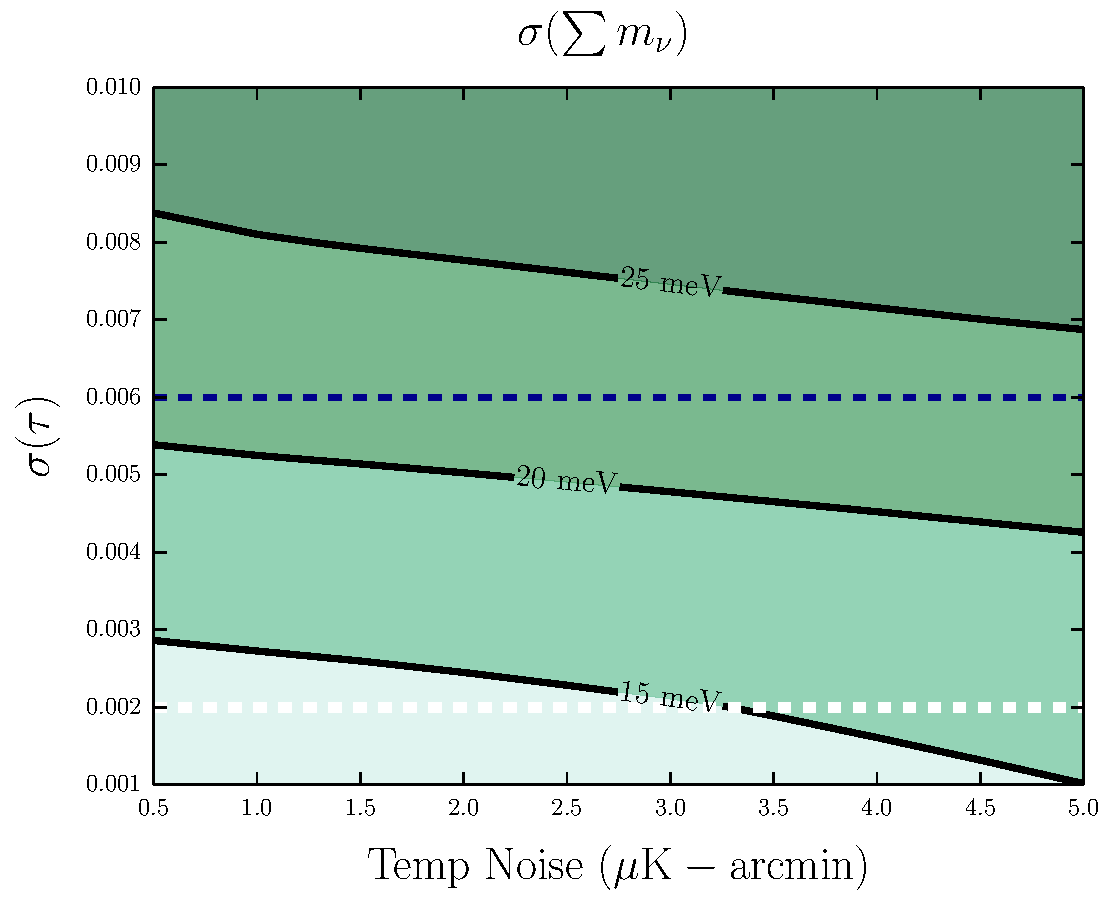
\includegraphics[width=0.45\textwidth]{figs/Mnu_tauprior.pdf}
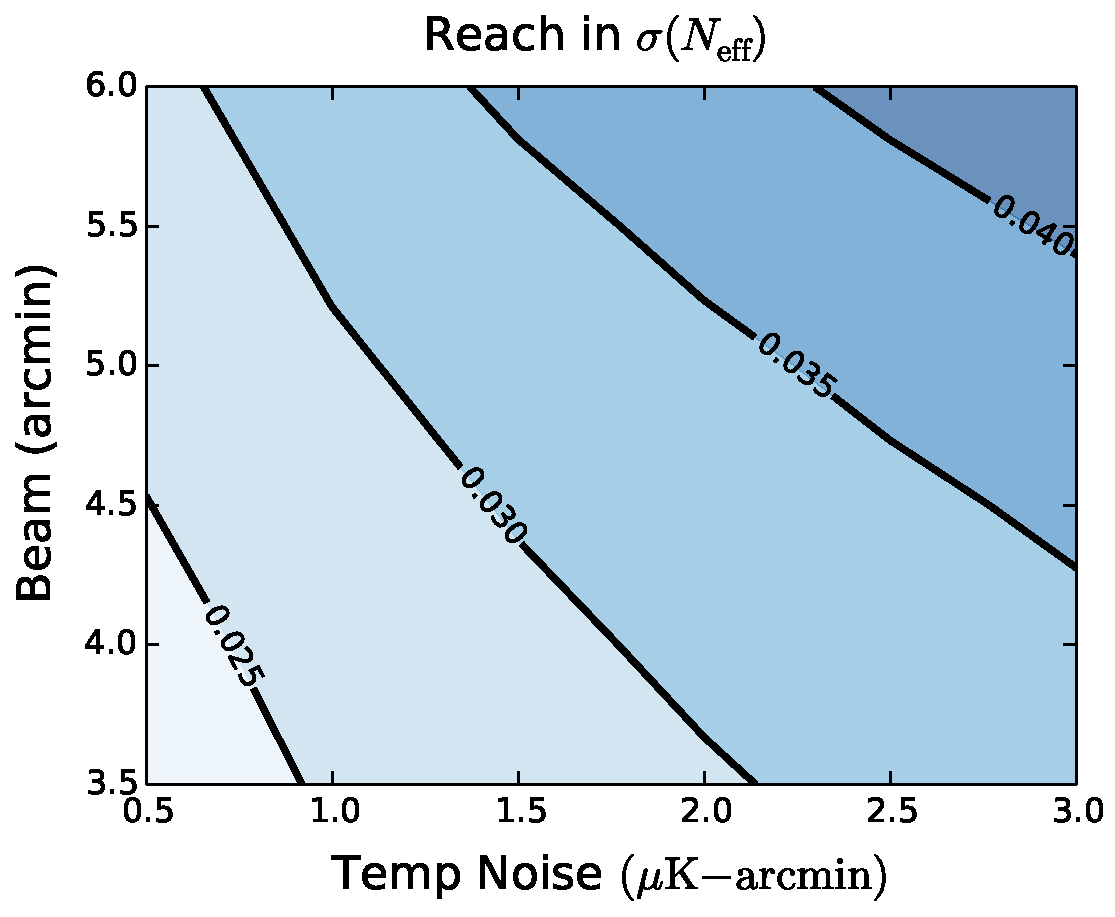
\includegraphics[width=0.45\textwidth]{figs/Neff_space.pdf}
\caption{ [Placeholders] {\it Left:} Neutrino mass constraints as a function of the prior on $\tau$.  {\it Right} $\Neff$ Forecasts as a function of resolution in arc-min and temperature noise in $\mu$K-arcmin assuming $f_{\rm sky} = 0.7$.}
\label{fig:Neff_future}
\end{center}
\end{figure}


\vspace{-0.22in}

\subsubsection{Other Science Goals (Spectrum, Lensing, ...)}

\comred{Here we write about other science goals. This structure -- inflation and 'other' -- is temporary. }

\vspace{-0.05in}

\subsection{The Challenges: Foregrounds, systematics}
\label{sec:foregrounds}

\vspace{-0.05in}

\comred{3 pages. Discuss the challenge of Foregrounds and Systematics. }
% Jo, Aurelien? 
\subsection{Current and Forthcoming Efforts and the CMB Probe}
\label{sec:spacemission}

\vspace{-0.05in}

\comred{2.5 pages. S3 experiments, forthcoming S4, Baselines CMB Probe options and their complementarity with S4.}
% Al, Shaul
\vspace{-0.22in}

\subsection{State of Technologies}
\label{sec:technologies}

\vspace{-0.05in}

\comred{2 pages. Discuss the technologies, their TRL, and what will be studied }
% Jamie, Adrian

\vspace{-0.22in}

\subsection{Mission Study, and Management Plan  }
\label{sec:management}

\vspace{-0.05in}

\comred{1.5 pages; Describe what we want to do, who is doing what, what we are funding}
% Shaul

\newpage

\bibliography{mybib}

\newpage
\section{Curriculum Vitae}
\label{sec:cv}

\newpage
\addtocounter{page}{8}
\section{Summary of Work Effort}
\label{sec:workeffort}

%:personnel 


\section{Current and Pending Support}
\label{sec:current_and_pending}

\newpage
\addtocounter{page}{13}
\section{Letters of Support}
\label{sec:lettersofsupport}

\newpage
\addtocounter{page}{3}
\section{Budget Details - Narrative}
\label{sec:budget}

\subsection{Team, and Work Effort}
\label{sec:budget_principles}


\subsubsection{Funded Team Members}

%Table~\ref{tab:tasks} delineates the allocation of task within the project. 

\subsubsection{Non-Funded Team Members}


\subsection{Costing Principles}
\label{sec:cost_principles}


$\bullet$ \hspace{0.2in} {\bf Summer Salaries:} 


$\bullet$ \hspace{0.2in} {\bf Workshop:} 


        \subsection{University of Minnesota Budget}


            \subsubsection{Direct Labor} 


            \subsubsection{Supplies} 

  
            \subsubsection{Travel} 


   \subsubsection{Other Direct Costs} 

{\bf Publications and Teleconferencing} \hspace{0.1in} 


{\bf Other Subcontracts} \hspace{0.1in} 

   \subsubsection{Facilities and Administrative Costs} 


\newpage
%\addtocounter{page}{9}

\section{Budget Sheets}

\end{document}

%\begin{table}[h] %%[h]
%\begin{center}
%\begin{tabular}{|c|c|c|c|c|c|} \hline 
%\multicolumn{6}{|c|}{Summary of Personnel and Work Efforts, (Page 1 of 2)}              \\ \hline
%Personnel & \multicolumn{5}{c|}{Budgeted Effort/Year (months)}  \\ \cline{2-6}
%                 & Year 1  & Year 2 & Year 3 & Year 4   & Year 5   \\ \hline
%\multicolumn{6}{|c|}{\textcolor{blue}{University of Minnesota } }              \\ \hline
%Hanany,  PI              & 1/1  & 1/1 & 1/1 & 1/1 & 1/1  \\ \hline
%\multicolumn{6}{|c|}{\textcolor{blue}{Cal Tech } } \\ \hline
%Jamie Bock, Co-I           &  0.25  & 0.25 & 0.25 & 0.25 & 0.25  \\ \hline
%\multicolumn{6}{|c|}{\textcolor{blue}{Princeton} }  \\ \hline
%Lyman Page, Co-I           & 1/1  & 1/1  & 1/1  & 1/1   & 1/1  \\ \hline
%\multicolumn{6}{|c|}{\textcolor{blue}{Goddard Space Flight Center } }  \\ \hline
%Al Kogut, Co-I               & 0.75 & 0.75 & 0.75 & 0.75  & 0.75   \\ \hline
%\multicolumn{6}{|l|}{ $^{1}$ PDR = Post-Doctoral Researcher; } \\ 
%\multicolumn{6}{|l|}{ $^{2}$ GSRA = Graduate Student Research Assistant;  } \\ \hline
%\end{tabular}
%\end{center}
%\vspace{-0.2in}
%\caption{ Personnel, time in months on the project funded by NASA/time in months on the project not funded by NASA, and their role.  When 
%only one time value appears it is time funded by NASA.  {\bf Continued on next page}.
%\label{tab:personnel} }
%\end{table}

%\newpage

%\begin{table}[h] %%[h]
%\begin{center}
%\begin{tabular}{|c|c|c|c|c|c|} \hline 
%\multicolumn{6}{|c|}{Summary of Personnel and Work Efforts, (Page 2 of 2)}              \\ \hline
%Personnel & \multicolumn{5}{c|}{Effort/Year (Months)}  \\ \cline{2-6}
%                 & Year 1  & Year 2 & Year 3 & Year 4    &  Year 5    \\ \hline
%\multicolumn{6}{|c|}{\textcolor{blue}{Johns Hopkins} }  \\ \hline
%Chuck Bennett, Co-I               & 0.5 & 0.5 & 0.5 & 0.5  & 0.5   \\ \hline
%\multicolumn{6}{|c|}{\textcolor{blue}{NIST } }  \\ \hline
%Hubmayr, Co-I    &  0/0.25 & 0/0.25 & 0/0.25 & 0 &  0 \\ \hline
%\multicolumn{6}{|c|}{\textcolor{blue}{Lawrence Berkeley National Lab} }  \\ \hline
%Borrill, Collaborator   &  0  &  0  & 0 & 0 & 0  \\ \hline
%\end{tabular}
%\end{center}
%\vspace{-0.1in}
%\end{table}

%\newpage
%\addtocounter{page}{8}


%%%%%%%%%%%%%%%%%%%%%%%%%%%%%%%%%%%%%%%%%%%%%


%\begin{figure}%[thbp!]
%\hspace{-0.35in}
%\parbox{2.2in}{ \centerline {
%\includegraphics[height=2.2in] {Figures/GondolaZoom}} }
%\hspace{0.in}
%\parbox{2.2in}{ \centerline {
%\includegraphics[height=2.3in] {Figures/ebexmodel2016}} }
%\hspace{0.in}
%\parbox{2.2in}{ \centerline {
%\includegraphics[height = 2.in]{Figures/RayTrace_current}}}
%\vspace{-0.15in}
%\caption{ \small \setlength{\baselineskip}{0.90\baselineskip}
%	{\bf Left Panel}: The \ebextw\ experiment on the launch pad in Antarctica prior to its long duration flight. 
%	{\bf Middle and Right Panels:} A solid model with major gondola
%	elements and overview of the optical system for \ebexsk ; see also Fig.~\ref{fig:ebexskfocalplane}. 
%	Relative to \ebextw\ the sun-shade structure will change and the solar panels 
%	will be mounted on the side to allow observations of the BICEP2 region.
%	\label{fig:ebexpreflight} }   
%\vspace{-0.1in}
%\end{figure}

%\begin{table} 
%\begin{center} 
%\begin{tabular}{|c|c|c|c|c|c|c|} \hline \hline
%Task        & Gondola    & \multicolumn{2}{c|} {Optics + Receiver}     & Detectors & \multicolumn{2}{c|}{ Readout}  \\ 
%\hline
%Task Leader & {\it Johnson + Tucker$^{1}$ } & \multicolumn{2}{c|} {\it Hanany+McMahon} & {\it Lee} & \multicolumn{2}{c|}{\it Dobbs} \\
%\hline
%Institution & {\it Columbia + Brown$^{1}$ } & \multicolumn{2}{c|}{\it UMN+Michigan}  & {\it UCB} & \multicolumn{2}{c|}{\it McGill}   \\ 
%\hline \hline 

%Task   &  \multicolumn{2}{c|}{Attitude Control }   &  IR Filters & Foregrounds & \multicolumn{2}{c|}{Theory + Analysis}  \\ 
%\hline
%Task Leader & \multicolumn{2}{c|}{\it Miller  } & {\it Ade + Tucker} & {\it Baccigalupi} &\multicolumn{2}{c|}{Stompor, Jaffe} \\  \hline
%Institution & \multicolumn{2}{c|}{\it Columbia } & {\it Cardiff} & {\it SISSA} &\multicolumn{2}{c|}{APC - Paris, Imperial }   \\  \hline \hline 
%\multicolumn{7}{|l|}{$^{1}$ {\footnotesize Brown contributes specific separable elements to the gondola hardware} } \\  \hline \hline 
%\end{tabular}
%\vspace{-0.1in}
%\caption{\footnotesize \setlength{\baselineskip}{0.95\baselineskip}
%	Tasks and task leaders and institutions for the EBEX project. }
%\label{tab:tasks}
%\end{center}
%\vspace{-0.25in}
%\end{table}


%\begin{table}[h]
%%\hspace{-0.2in}
%\begin{center}
%\begin{tabular}{cccccc} 
%\hline \hline
%Pixel & Center Frequency & FWHM & NET/detector & Detectors & Array NET \\
% Type & (GHz) & (arcmin) &   (\microkrtsec)$^{a}$  & (\#) & (\microkrtsec)$^{a}$  \\ 
%   \hline
%          \multirow{2}{*}{Low Frequency}    & 150/180$^{b}$ & 7.2/6.0  & 142/148  & 2316/2316  & 2.95/3.08 \\
%          \multirow{2}{*}{(2316 pixels)}    & 250 & 4.4  & 248  & 3202  & 4.38 \\  
%                                            & 320 & 3.6  & 498  & 2648  & 9.68 \\  
%   \hline
%           \multirow{2}{*}{High Frequency}  & 220 & 4.9  & 219  & 3360  & 3.78 \\    
%           \multirow{2}{*}{(1680 pixels)}   & 280 & 3.9  & 361  & 3360  & 6.23 \\ 
%                                            & 360  & 3.2  & 956 & 3360  & 16.5 \\ 
%   \hline
%          Total                             &    &      &       & 20562 &      \\
%   \hline
%\multicolumn{4}{l}{$^{a}$ {\small Thermodynamic units; multiply by $\sqrt{2}$ for Stokes $Q,U$}} \\
%\multicolumn{6}{l}{$^{b}$ {\small Half of the pixels are with 150~GHz, the other half with 180~GHz (see Section~\ref{sec:detectors}) }} \\ \hline \hline
%\end{tabular}
%\end{center}
%\vspace{-0.2in}
%\caption{\small \setlength{\baselineskip}{0.90\baselineskip}
%	Specifications of the \ebexsk\ focal plane multi-chroic pixels and detectors.  The calculation of incident optical power 
%	assumes a bandwidth $\Delta \nu / \nu = 23\%$ and includes all known
%	contributions: the CMB, atmosphere, warm mirror, warm vacuum window, filters, cold lenses, 
%	and cold half-wave plate.  Thermal noise is calculated assuming that the
%	thermal conductance of the TES is optimized for 2.5 times the 
%	absorbed optical power. TES absorption efficiencies are 
%	assumed to be 0.7, 0.7, 0.65, 0.6, 0.6, 0.55 and 0.50 for 150~GHz and higher bands, respectively. 
%	See Section~\ref{sec:detectors} for more details on the focal plane layout.}
%\label{tab:band_sens}
%\vspace{-0.1in}
%\end{table}
%\vspace{-0.1in}
%\noindent\rule{6.5in}{0.4pt}
%%\vspace{-0.15in}


